\section{Global Infrastructure}\label{sec:global-infrastructure}

\subsection{Why make a global application?}\label{subsec:why-make-a-global-application}

\begin{itemize}
    \item{\textbf{Standard - General Purpose}: 99.99\% available.}
    \item{\textbf{Deployed in multiple geographies:}} Regions and Edge Locations.
    \item{\textbf{Decreases latency:}} Deploy applications closer to users.
    \item{\textbf{Disaster recovery:}} Fail-over to another region.
    \item{\textbf{Attack protection:}} Harder to attack.
\end{itemize}

\subsection{Components}\label{subsec:global-application-components}

\begin{figure}[h]
    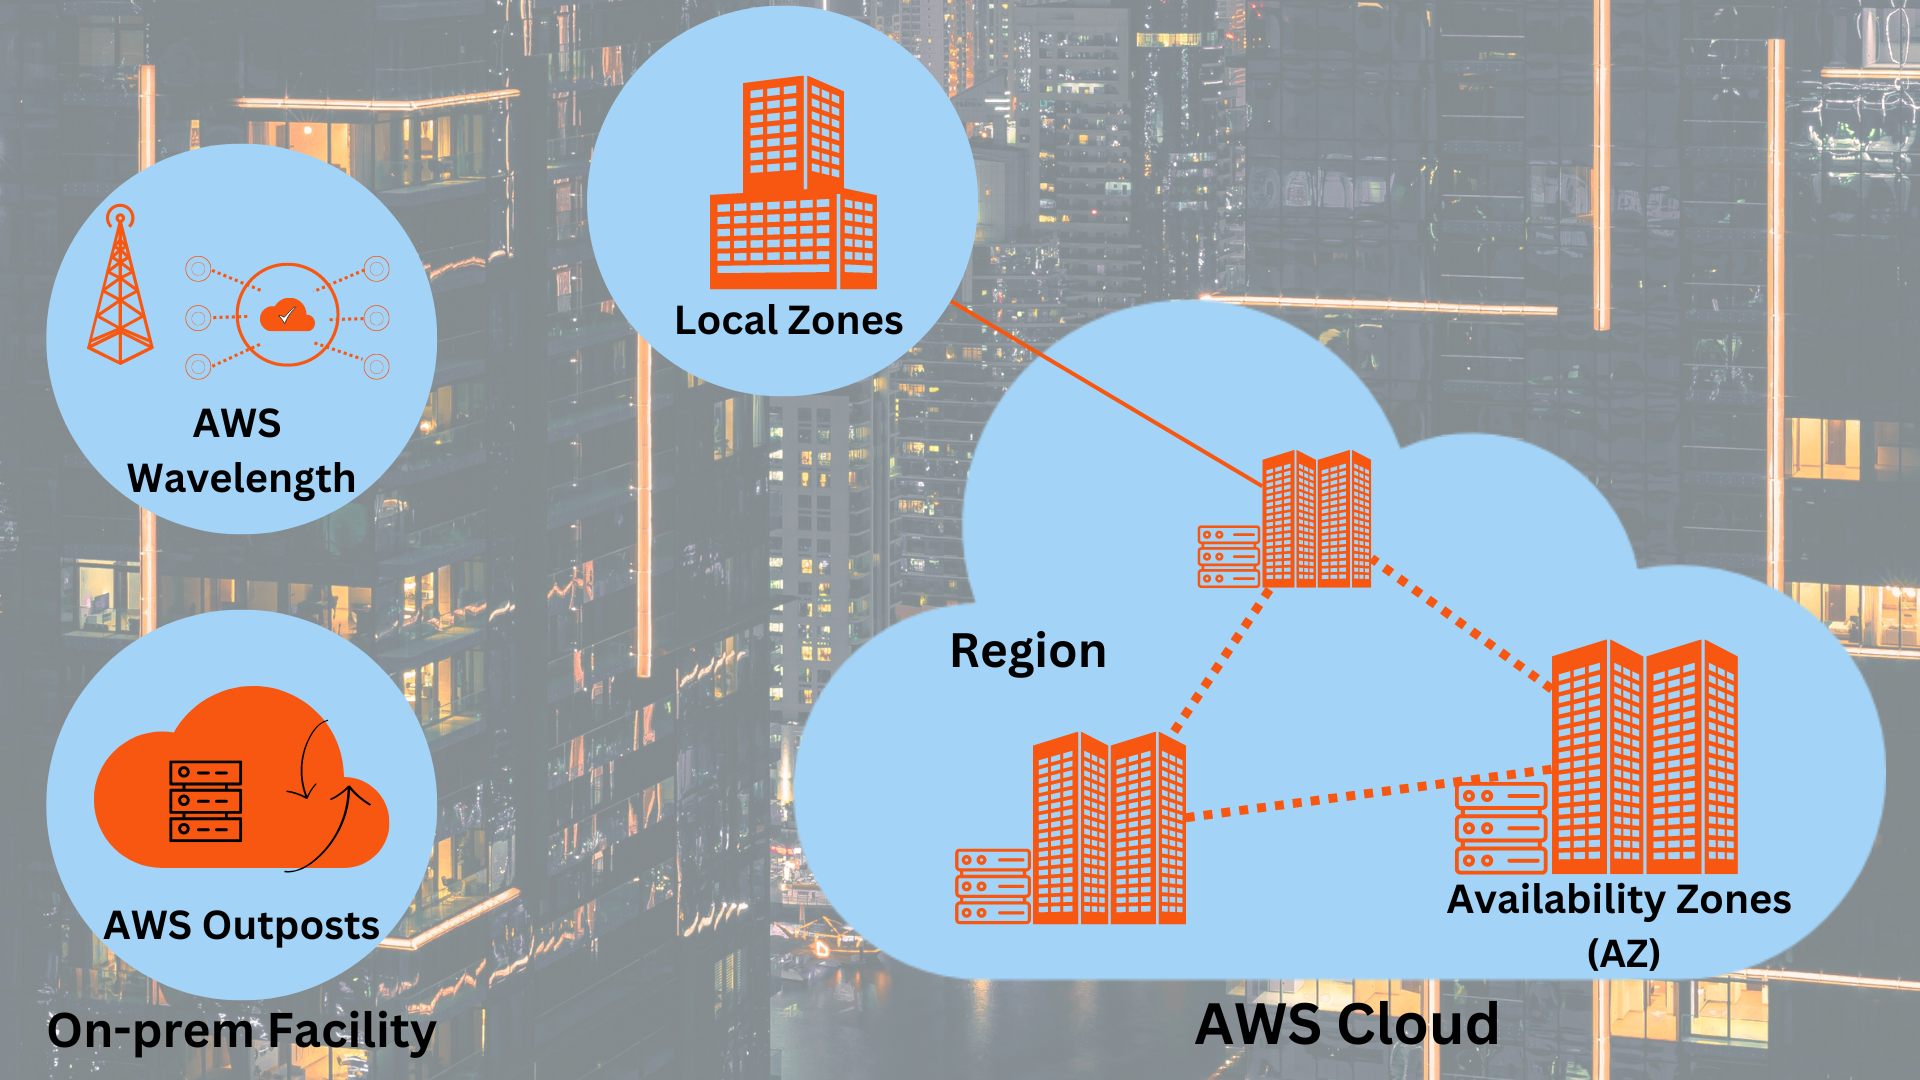
\includegraphics[scale=0.20]{global-infrastructure/global-infrastructure}
    \centering
    \label{fig:global-infrastructure}
\end{figure}

\subsection{Global AWS applications}\label{subsec:global-aws-applications}

\subsubsection{Route 53}
Managed DNS\@.

\subsubsection{Cloudfront}
Content Delivery Network (CDN).
Improves read performance because content is cached at an edge location.
DDoS protection.

\subsubsection{S3 Transfer Acceleration}
Improve transfer speed by transferring to an edge location.

\subsubsection{Global Accelerator}
Improve global application availability and performance by using the AWS internal network through edge location.

\subsubsection{Outpost}
On-premise local private AWS infrastructure.

\subsubsection{WaveLength}
Infrastructure embedded within telcom providers datacenter at the edge of the 5G networks.

\subsubsection{Local Zones}
Places AWS resources closer to end users (reduce latency).
